\documentclass[12pt]{standalone}
\usepackage{tikz}
\usetikzlibrary{decorations.pathreplacing, calc, arrows.meta}

\begin{document}
%
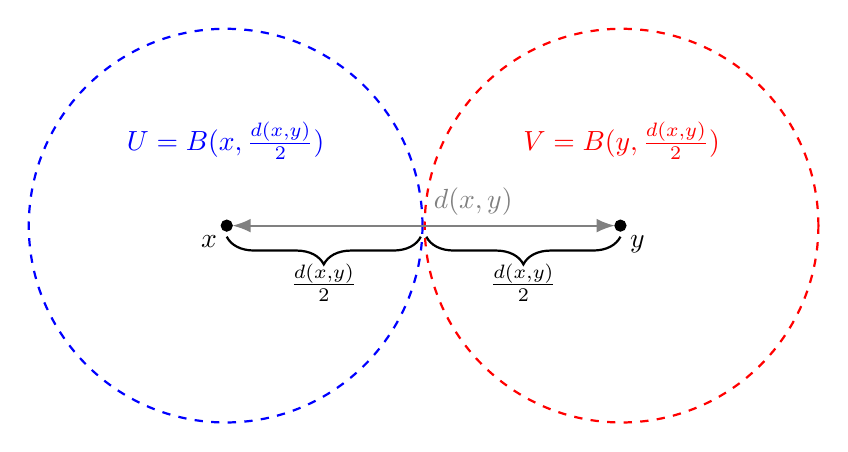
\begin{tikzpicture}[baseline={(0,0)}]

\def\distance{5}  % Distance between x and y

% Define the coordinates of the points
\coordinate (x) at (0,0);
\coordinate (y) at (\distance,0);  % d(x, y) = 5

% Define radii for the open balls around x and y (both equal to d(x, y) / 2)
\def\radius{\distance/2}  % Set r1 = r2 = d(x, y) / 2

% Draw the open balls as circles with dashed boundaries
\draw[blue, thick, dashed] ($ (x) + (-0.4pt, 0) $) circle (\radius) node[above=20pt] {$U=B(x, \frac{d(x,y)}{2})$};
\draw[red, thick, dashed] ($ (y) + (0.4pt, 0) $) circle (\radius) node[above=20pt] {$V=B(y, \frac{d(x,y)}{2})$};

% Draw the points x and y
\filldraw[black] (x) circle (2pt) node[below left] {$x$};
\filldraw[black] (y) circle (2pt) node[below right] {$y$};

% Draw the line connecting x and y
\draw[thick, gray, {Latex}-{Latex}, shorten <= 2pt, shorten >= 2pt] (x) -- (y) node[midway, above right] {$d(x, y)$};

% Add braces to show that r1 = r2 = d(x, y) / 2
\draw[decorate,decoration={brace,amplitude=10pt,mirror,raise=4pt},  thick] 
  (x) -- ($ (x) + (\radius,0) + (-1pt, 0) $) node[midway, below=10pt] {$\frac{d(x,y)}{2}$};
\draw[decorate,decoration={brace,amplitude=10pt,mirror,raise=4pt}, thick] 
  ($ (y) + (-\radius,0) + (1pt, 0) $) -- (y) node[midway, below=10pt] {$\frac{d(x,y)}{2}$};

\end{tikzpicture}
\end{document}
